
\begin{SCfigure*}
	\centering
	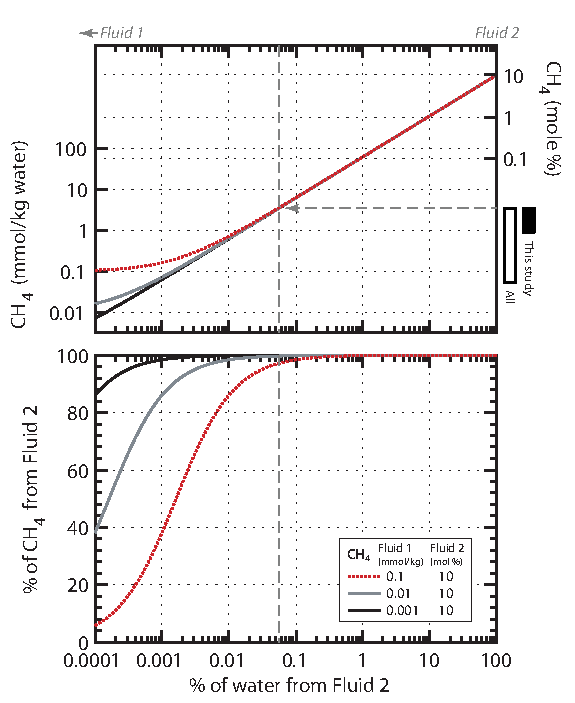
\includegraphics[width=0.65\linewidth]{figures/Fig3.6}
	\caption[Concentration of CH\textsubscript{4} in hydrothermal fluids upon mixing of a CH\textsubscript{4}-rich crustal fluid with a circulating, CH\textsubscript{4}-poor fluid]{%
		Composition
		of fluids formed by mixing of a CH\textsubscript{4}-poor
		actively-circulating seawater-derived hydrothermal fluid
		(\emph{Fluid~1}) with a CH\textsubscript{4}-rich fluid such as those
		observed in inclusions in plutonic rocks on the Southwest Indian Ridge
		and on the Mid-Atlantic Ridge (\emph{Fluid~2}) \parencite{Kelley_1996_JGR,Kelley_1997,Kelley+FruhGreen_1999_JGR}. Mixing curves are plotted for
		CH\textsubscript{4} concentrations in the \emph{Fluid~1} endmember
		ranging from 1 to 100~µmol/kg. Calculations assume that molalities of
		species other than CH\textsubscript{4} have a negligible effect on mole
		fractions in the high-CH\textsubscript{4} fluid. The black and white
		bars show CH\textsubscript{4} concentrations in vent fluids from this
		study (\autoref{tab:3:2}) and from mid-ocean ridge hydrothermal systems globally
		\parencite{Keir_2010_GRL}.
	}
	\label{fig:3:6}
\end{SCfigure*}



